The IDDR implementation uses the \texttt{Linux kernel 3.5.0} for both application domain and driver domain. We tested it with Arch Linux on \texttt{x86\_64} platform. The specification of the system used for evaluation is presented in the table~\ref{tab:config}. 

\begin{table}
\caption{Specifications of the system}
%\begin{center}
\begin{tabular}{ll}
  \hline
  \label{tab:config}
  System Parameter & Configuration \\
  \hline
  Processor & 1 X Quad-code AMD Opteron(tm) Processor 2380, 2.49 Ghz \\
  Number of cores & 4 per processor \\
  Hyperthreading & OFF \\
  %Turbo boost & ?? \\
  L1 L2 cache & 64K/512K per core \\
  L3 cache & 6144K \\
  Main memory & 16Gb \\
  Storage & SATA, HDD ??RPM \\
  \hline 
\end{tabular}
%\end{center}
\end{table}
 

\section{Goals}
\label{sec:goals}
Our evaluation contains 
\begin{enumerate} 
\item comparison of the Xen's isolated driver domain with baseline IDDR system, 
\item an evaluation of IDDR performance improvement over base IDDR system,
\end{enumerate}
The first goal of the evaluation is to verify and compare the performance of the baseline IDDR system with that of the Xen's isolated driver domain. The comparison shows that the performance of the IDDR system matches the performance of the Xen's isolated driver domain. 
\\[3mm] 
The second goal is to show that the performance of the IDDR system improves if a frontend and backend driver spins over a spinlock to check the availability of requests and responses, instead of sending event channel interrupts to notify the availability of requests and responses. 

\section{Methodology}
In a Linux system, a loop device is a device that makes a file accessible as a block device. A ramdisk is a block of a memory, which acts as a disk drive. We use block devices such as SATA disk, ramdisk and loop device for the performance testing. These devices cover the variety of block devices we would want to test our system against.
\\[3mm]
In order to measure performance, we format the block device with the ext2 file system, and run the fileIO SysBench benchmark~\cite{sysbench} on it. SysBench is a multi-threaded benchmark tool for evaluating a system. It evaluates the system performance without installing a database or without setting up complex database benchmarks. Sysbench benchmark has different test modes. FileIO is one of the test mode which can be used to produce various file I/O workloads. SysBench can run a specified number of threads by executing all requests in parallel. Sysbench benchmark in fileIO test mode generates 128 files with \texttt{1Gb} of total data and performs random reads, random writes and mix of random read-writes with a block size of \texttt{16Kb}. 

\section{Xen split driver vs IDDR}
The IDDR system is a re-implemention of the Xen's isolated driver domain. We improve the performance of the base IDDR system by introducing spinlocks instead of the event channel interrupts in the communication channel. As per our first goal of evaluation mentioned in Section~\ref{sec:goals}, we compare the baseline IDDR with the Xen's isolated driver domain. In this comparision, we show that the performance of the base IDDR system matches the Xen's isolated driver domain. This verifies the baseline performance of the IDDR.
\\[3mm]
As explained in chapter 2, Xen's isolated driver domain follows the architecture of the Xen split driver. In order to measure the performance of the Xen's isolated driver domain, we run performance benchmarks on a block device which uses the Xen split driver.

\subsection{Experimental setup}

\subsubsection*{Xen split driver}
We create a ramdisk in domain 0. The guest domain domU is configured such that the ramdisk uses a split device driver and the ramdisk is available in the guest domain. We do a similar setup for the loop device and the SATA disk. For example, in case of loop device, we create a loop device in domain 0 and then configure the guest domain to use the loop device as a disk. In case of SATA disk, we configure the guest domain to use SATA disk as a secondary disk. We format and mount the disk in the guest domain with the ext2 file system. Sysbench benchmark is run on the mounted partition as explained in section~\ref{sec:goals}.

\subsubsection*{IDDR}
In the Xen split device driver setup, the backend device driver runs in a domain 0 and the frontend device driver runs in the domain U. 
\\[3mm]
Xen paravirtualized guests are aware of the VMM and require special ported kernel to run on Xen VMM, so the guests can run efficiently without emulation or virtual emulated hardware. Paravirtualization does not require virtualization extensions from the host CPU. 
\\[3mm]
Fully virtualized or Hardware Virtual Machine (HVM) guests require CPU virtualization extensions such as Intel VT, AMD-V. The Xen uses modified version of Qemu to emulate hardware for HVM guests. CPU virtualization extensions are used to boost performance of the emulation. Fully virtualized guests do not require special kernel. In order to boost performance fully virtualized HVM guests use special paravirtual device drivers to bypass the emulation for disk and network IO.
\\[3mm]
Our setup is configured such that the domain U is a HVM guest and the domain 0 is a PV guest. HVM guests are expected to have less syscall overhead and faster memory bandwith than PV guests. In order to have a fair comparision, it is necessary to run the backend driver of the IDDR system in the domain 0 and the frontend driver of the IDDR system in the domain U.
\\[3mm]
We insert a ramdisk and the IDDR frontend module in the domain 0. The IDDR backend module is inserted in the guest domain domU. We format and mount the ramdisk with ext2 file system and sysbench benchmark is run on it.  
\\[3mm]
Similar setup is used for loop device and SATA disk.
\subsubsection*{Comparision}
Figure~\ref{fig:iddrvsxen-ramdisk-rdwr} shows the performance of random reads-writes on a ramdisk, and Figure~\ref{fig:iddrvsxen-loop-rd} shows the performance of random reads on a loop device. Both systems provide roughly similar performance. The figures show that the performance of the IDDR matches the performance of the Xen's isolated driver domain. 
\begin{figure}[!ht]
\centering
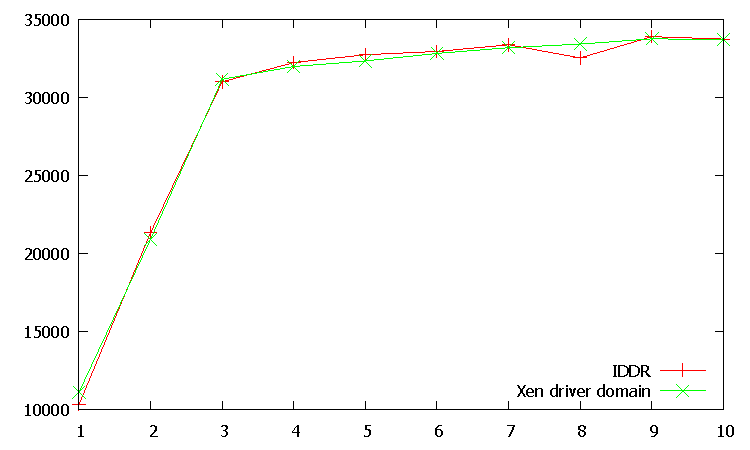
\includegraphics[scale=1]{iddrvsxen-ramdisk-rdwr}
\caption{IDDR vs Xen split driver}
\label{fig:iddrvsxen-ramdisk-rdwr}
\end{figure}
\begin{figure}[!ht]
\centering
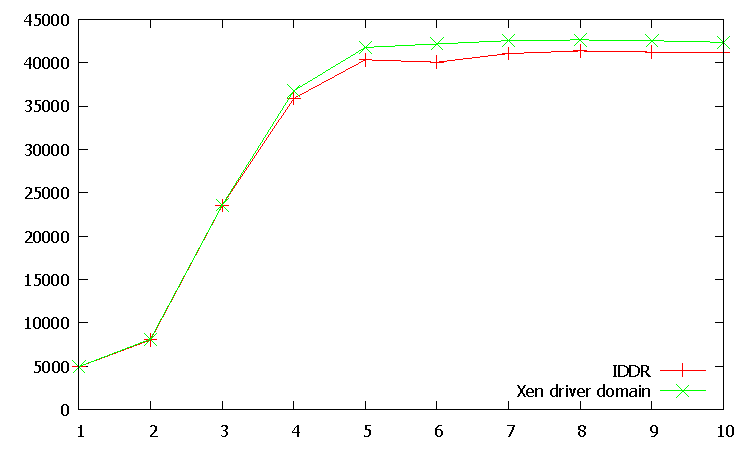
\includegraphics[scale=1]{iddrvsxen-loop-rd}
\caption{IDDR vs Xen split driver}
\label{fig:iddrvsxen-loop-rd}
\end{figure}

\section{IDDR performance improvement}
We measure and compare the performance of the base IDDR system (event channel interrupt) with the new IDDR system with spinlock. We run the fileIO sysbench benchmark with random reads, random writes and mixed random reads-writes. 
\subsection{Experimental setup}
In the setup, domain 0 is an application domain, and domain U is a driver domain. A ramdisk is created in the domain U (driver domain). The backend driver is inserted in the domain U (driver domain) and the frontend driver is inserted in the domain 0 (application domain). The disk is formatted and mounted with ext2 file system in the application domain. Sysbench benchmark is run on the mounted partition. 
\\[3mm]
For loop device a similar setup is used where we create a loop device in a driver domain, and insert the backend driver in the driver domain. The front end driver is inserted in domain 0. For SATA disk, we passthrough SATA disk to driver domain, so that the driver domain can directly access the SATA disk. 
\subsubsection*{Comparision}
Figure~\ref{fig:threadvsspinram} compares the performance of the base IDDR and the new IDDR with random reads-writes on a ramdisk. The figure shows that the new IDDR system implementation with spinlock performs better than the base IDDR implementation. 
\begin{figure}[!ht]
\centering
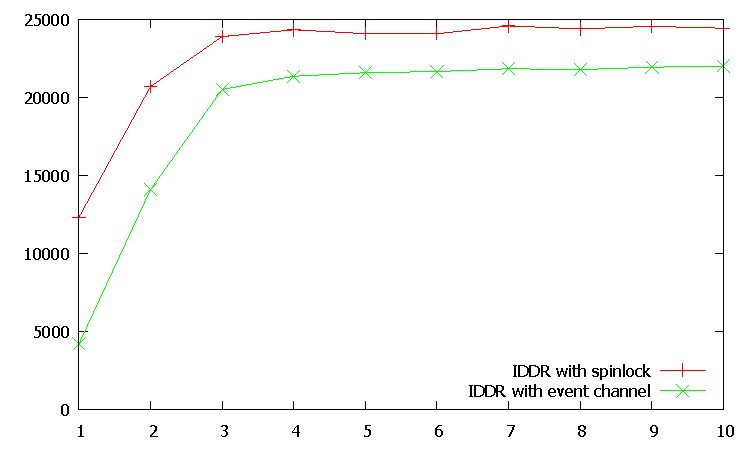
\includegraphics[scale=1]{threadvsspinram}
\caption{IDDR with Spinlock vs IDDR with event channel (ramdisk)}
\label{fig:threadvsspinram}
\end{figure}



\subsubsection*{Comparision}
Figure~\ref{fig:threadvsspinloop} compares the performance of the base IDDR and the new IDDR with random reads on a loop device. The figure shows that the new IDDR system implementation with spinlock performs better than the base IDDR implementation. 
\begin{figure}[!ht]
\centering
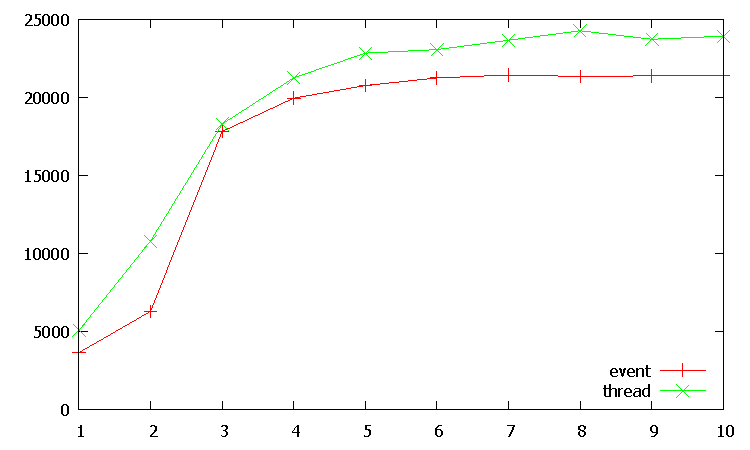
\includegraphics[scale=1]{threadvsspinloop}
\caption{IDDR with Spinlock vs IDDR with event channel (loop device)}
\label{fig:threadvsspinloop}
\end{figure}


% ref
\ifbool{toShowBibliography}{\bibliography{references}}{}